\documentclass[11pt]{article}
\usepackage[a4paper,margin=1in]{geometry}
\usepackage{amsmath,amssymb,amsthm}
\usepackage{graphicx}
\usepackage[hidelinks]{hyperref}
\setlength{\emergencystretch}{3em}

\newtheorem{theorem}{Theorem}
\newtheorem{lemma}{Lemma}
\newtheorem{corollary}{Corollary}
\newtheorem{remark}{Remark}

\newcommand{\ddc}{dd^c}
\newcommand{\psh}{\operatorname{psh}}
\newcommand{\qpsh}{\operatorname{qpsh}}
\newcommand{\co}{\operatorname{co}}

\title{Normability of Higher Complex Sobolev Quasinorms}
\author{Automatic math-discovery packet}
\date{July 3, 2026}

\begin{document}
\maketitle

\section*{Source Question}

The source paper is Thai Duong Do and Duc-Bao Nguyen,
\emph{Higher complex Sobolev spaces on complex manifolds}, arXiv:2405.06385.
In Remark 2.4, after defining the \(q\)-star quasinorm
\(\|\cdot\|_{*,q}\) on the higher complex Sobolev spaces \(W_q^*\), the
authors ask whether there is an equivalent norm. The relevant passage is:

\begin{quote}
It is interesting to know if we can build a norm in \(W_q^*\) equivalent to
\(\|\cdot\|_{*,q}\). When \(q\geq2\), since the mass of elements in the
defining sequence can be chosen independently with each other [...] it seems
to us that such a norm does not exist.
\end{quote}

\begin{figure}[h]
\centering
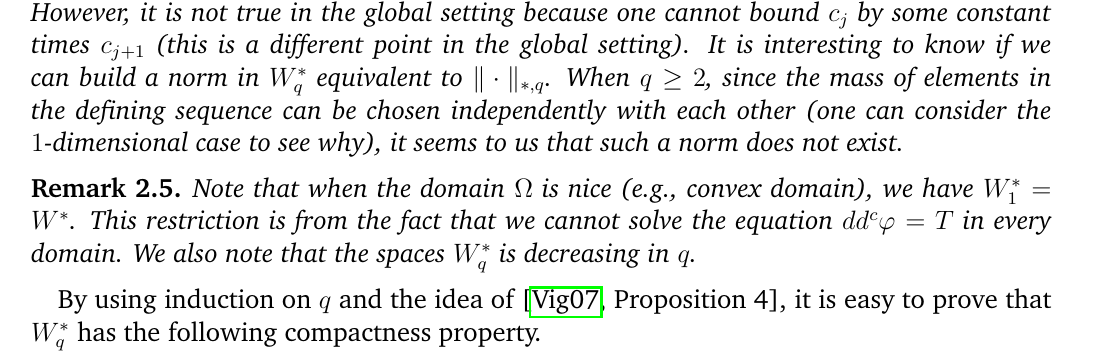
\includegraphics[width=\textwidth]{figures/remark_2_4_normability_question_crop.png}
\caption{Remark 2.4 in the source paper, page 8.}
\end{figure}

\section*{Claim}

The answer is positive. For every \(q\geq1\), in both the local and global
settings of the source paper, \(W_q^*\) admits a norm equivalent to
\(\|\cdot\|_{*,q}\). More concretely, if
\[
  B=\{\varphi\in W_q^*: \|\varphi\|_{*,q}\leq1\},
\]
then \(\co(B)\) is bounded for \(\|\cdot\|_{*,q}\). Hence the Minkowski
functional of \(\co(B)\) is an equivalent norm.

\section*{Definitions}

In the local setting, \(\Omega\subset\mathbb C^k\) is a bounded domain. A
defining sequence for \(\varphi\in W_q^*(\Omega)\) is a sequence of psh
functions \((\varphi_1,\ldots,\varphi_q)\), with \(\varphi_0=\varphi\), such
that
\[
  d\varphi_{j-1}\wedge d^c\varphi_{j-1}\leq \ddc\varphi_j,
  \qquad j=1,\ldots,q,
\]
and the masses \(\|\ddc\varphi_j\|\) are finite. The quasinorm is
\[
  \|\varphi\|_{*,q}
  =\|\varphi\|_{L^2(\Omega)}
   +\inf \sum_{j=1}^q \|\ddc\varphi_j\|^{1/2^j}.
\]

In the global setting, \((X,\omega)\) is a compact K\"ahler manifold. A
defining sequence for \(\varphi\in W_q^*(X)\) is
\(((c_1,\varphi_1),\ldots,(c_q,\varphi_q))\), where \(c_j\geq0\) and
\(\varphi_j\) are qpsh, such that
\[
  d\varphi_{j-1}\wedge d^c\varphi_{j-1}
  \leq c_j\omega+\ddc\varphi_j,
  \qquad j=1,\ldots,q.
\]
The quasinorm is
\[
  \|\varphi\|_{*,q}
  =\|\varphi\|_{L^2(X)}
   +\inf \sum_{j=1}^q c_j^{1/2^j}.
\]

\section*{Proof Intuition}

The possible obstruction in Remark 2.4 is that the different levels of a
defining sequence are not controlled by each other in the global setting. But
normability does not require such interlevel control. It is enough to show
that the convex hull of the quasinorm unit ball remains bounded.

Inside the unit ball, every individual level is bounded: each
\(\|\ddc\varphi_j\|\), or each \(c_j\), is at most one. If we take a convex
combination of functions, we take the same convex combination of their
defining sequences. Convex combinations preserve psh/qpsh functions, and the
basic Jensen inequality
\[
  d\Big(\sum_i \theta_i u_i\Big)\wedge d^c\Big(\sum_i \theta_i u_i\Big)
  \leq \sum_i \theta_i\,du_i\wedge d^cu_i
\]
preserves the defining inequalities level by level. Therefore each level of a
convex combination still has mass or constant at most one. The resulting
quasinorm bound is at most \(q+1\), uniformly over the whole convex hull.

\section*{Levelwise Convexity Lemma}

\begin{lemma}
\label{lem:jensen}
Let \(\theta_i\geq0\), \(\sum_i\theta_i=1\), and let \(u_i\in W^{1,2}\) be
real-valued. Then, in the sense of positive \((1,1)\)-currents,
\[
  d\Big(\sum_i \theta_i u_i\Big)\wedge d^c\Big(\sum_i \theta_i u_i\Big)
  \leq \sum_i \theta_i\,du_i\wedge d^cu_i .
\]
\end{lemma}

\begin{proof}
For smooth functions this is the pointwise Hilbert-space inequality
\[
  \left|\sum_i \theta_i \xi_i\right|^2\leq \sum_i\theta_i|\xi_i|^2
\]
applied to the complex gradients. The general \(W^{1,2}\) case follows by
the same pointwise inequality for the a.e. defined weak gradients, hence in
the associated positive current sense.
\end{proof}

\section*{Main Theorem}

\begin{theorem}
\label{thm:normable}
For every \(q\geq1\), the quasinormed spaces \(W_q^*(\Omega)\) and
\(W_q^*(X)\) of the source paper are normable. More precisely, the Minkowski
functional of the convex hull of the \(\|\cdot\|_{*,q}\)-unit ball is a norm
\(\|\cdot\|_{\mathrm{cvx},q}\) satisfying
\[
  \|\varphi\|_{\mathrm{cvx},q}
  \leq \|\varphi\|_{*,q}
  \leq (q+1)\|\varphi\|_{\mathrm{cvx},q}.
\]
\end{theorem}

\begin{proof}
Write \(Q(\varphi)=\|\varphi\|_{*,q}\) and
\[
  B=\{\varphi:Q(\varphi)\leq1\}.
\]
Since \(Q\) is homogeneous, \(B\) is balanced. Hence \(U:=\co(B)\) is convex,
balanced, and absorbing. It remains to prove that \(U\) is \(Q\)-bounded.

We first treat the global setting. Let
\[
  \varphi=\sum_{i=1}^N\theta_i\varphi^{(i)},\qquad
  \theta_i\geq0,\quad \sum_i\theta_i=1,\quad Q(\varphi^{(i)})\leq1.
\]
For each \(i\), choose a defining sequence
\[
 ((c_{i,1},\varphi_{i,1}),\ldots,(c_{i,q},\varphi_{i,q}))
\]
for \(\varphi^{(i)}\) with
\[
  \|\varphi^{(i)}\|_{L^2}
  +\sum_{j=1}^q c_{i,j}^{1/2^j}\leq 1+\varepsilon.
\]
Define
\[
  \Phi_j=\sum_{i=1}^N\theta_i\varphi_{i,j},
  \qquad
  C_j=\sum_{i=1}^N\theta_i c_{i,j}.
\]
Convex combinations of qpsh functions are qpsh. By Lemma~\ref{lem:jensen}
and the defining inequalities for the \(\varphi^{(i)}\),
\[
\begin{aligned}
  d\Phi_{j-1}\wedge d^c\Phi_{j-1}
  &\leq \sum_i\theta_i\,
       d\varphi_{i,j-1}\wedge d^c\varphi_{i,j-1}  \\
  &\leq \sum_i\theta_i(c_{i,j}\omega+\ddc\varphi_{i,j})
   = C_j\omega+\ddc\Phi_j .
\end{aligned}
\]
Thus \(((C_1,\Phi_1),\ldots,(C_q,\Phi_q))\) is a defining sequence for
\(\varphi\). Moreover,
\[
  C_j\leq (1+\varepsilon)^{2^j}
\]
for every \(j\), because \(c_{i,j}^{1/2^j}\leq1+\varepsilon\). Also
\[
  \|\varphi\|_{L^2}\leq \sum_i\theta_i\|\varphi^{(i)}\|_{L^2}\leq1+\varepsilon.
\]
Consequently
\[
  Q(\varphi)
  \leq (1+\varepsilon)+\sum_{j=1}^q(1+\varepsilon)
  =(q+1)(1+\varepsilon).
\]
Letting \(\varepsilon\downarrow0\), \(Q(\varphi)\leq q+1\) for every
\(\varphi\in U\).

The local proof is identical. If
\((\varphi_{i,1},\ldots,\varphi_{i,q})\) are local defining sequences, set
\(\Phi_j=\sum_i\theta_i\varphi_{i,j}\). Lemma~\ref{lem:jensen} gives the
defining inequalities, and positivity of the currents gives
\[
  \|\ddc\Phi_j\|
  \leq\sum_i\theta_i\|\ddc\varphi_{i,j}\|
  \leq (1+\varepsilon)^{2^j}.
\]
The same \(q+1\) bound follows.

Now define
\[
  \|\varphi\|_{\mathrm{cvx},q}
  :=\inf\{t>0:\varphi\in tU\}.
\]
Because \(U\) is convex, balanced, and absorbing, this is a seminorm. The
bound \(Q\leq q+1\) on \(U\) makes it positive definite: if
\(\|\varphi\|_{\mathrm{cvx},q}=0\), then \(Q(\varphi)\leq(q+1)t\) for every
\(t>0\), so \(Q(\varphi)=0\) and \(\varphi=0\). Thus it is a norm.

Finally, since \(B\subset U\), homogeneity gives
\[
  \|\varphi\|_{\mathrm{cvx},q}\leq Q(\varphi).
\]
Conversely, if \(\varphi\in tU\), then \(Q(\varphi)\leq(q+1)t\). Taking the
infimum over \(t\) gives
\[
  Q(\varphi)\leq(q+1)\|\varphi\|_{\mathrm{cvx},q}.
\]
This proves the equivalence.
\end{proof}

\begin{corollary}
With the norm \(\|\cdot\|_{\mathrm{cvx},q}\), the spaces \(W_q^*(\Omega)\)
and \(W_q^*(X)\) are Banach spaces whenever they are complete for
\(\|\cdot\|_{*,q}\). In particular, this applies to the complete spaces in
Proposition 2.7 of the source paper.
\end{corollary}

\begin{proof}
Equivalent quasinorms/norms define the same Cauchy sequences. The source
paper proves completeness for \(\|\cdot\|_{*,q}\) in Proposition 2.7.
\end{proof}

\section*{Verification Notes}

The proof uses only three ingredients already present in the source setup:
homogeneity of the quasinorm, convexity of the classes of psh/qpsh functions,
and Jensen's inequality for squared Hilbert norms of gradients. The script
\texttt{code/verify\_convex\_bound.py} checks the finite-dimensional scalar
inequality and the levelwise \(q\)-bound in random samples. It is a sanity
check, not a substitute for the proof.

\section*{Limitations and Novelty Check}

The constructed norm is abstract: it is the Minkowski functional of the
convex hull of the quasinorm unit ball. It does not give a simple formula in
terms of a last defining-sequence mass, and it does not contradict the source
paper's observation that the proposed norm \(\|\cdot\|_{**,q}\) need not be
equivalent to \(\|\cdot\|_{*,q}\) in the global setting.

The run indexes were searched for arXiv:2405.06385, higher complex Sobolev
spaces, \(W_q^*\), \(q\)-star quasinorms, and normability. No prior packet was
found. A bounded web search on July 3, 2026 for the exact title, the exact
phrase ``It is interesting to know if we can build a norm'', and
\(W_q^*\)/complex Sobolev quasinorm terms located only the arXiv source paper
and no later answer.

\section*{References}

\begin{itemize}
\item T. D. Do and D.-B. Nguyen, \emph{Higher complex Sobolev spaces on
complex manifolds}, arXiv:2405.06385.
\item S. Rolewicz, \emph{Metric Linear Spaces}, PWN, 1985. Standard reference
for normability criteria of quasi-normed linear spaces. The proof above is
self-contained via the Minkowski functional.
\end{itemize}

\section*{Human Review Recommendation}

Check the current inequality in Lemma~\ref{lem:jensen} under the exact
normalization of \(d^c\) used in the source paper. The normalization cancels
on both sides, so no constant should appear, but this is the only convention
sensitive point. Also verify whether the source authors intended the question
only for the global spaces; the proof covers both global and local versions.

\end{document}
